% ======================================================================
%  SUPPLEMENTARY INFORMATION  (S-numbered figures and tables)
% ======================================================================
\clearpage
\setcounter{figure}{0}
\setcounter{table}{0}
\renewcommand{\thefigure}{S\arabic{figure}}
\renewcommand{\thetable}{S\arabic{table}}
\section*{Supplementary Information}

% ---------- Supplementary Fig S1 : zero-shot FM benchmark on MOVER ----------
\begin{figure}[H]
\centering

\includegraphics[width=\textwidth]{FigS_zeroshot_mover.png}
\caption{\textbf{External-cohort (MOVER) zero-shot foundation-model benchmark.}
TiRex-2 versus Chronos-Bolt, TimesFM-2.5 and Moirai-1.1-R on hypotension
AUROC, CRPS, calibration and AUPRC across horizons on the independent MOVER
cohort. The development-cohort ranking (Fig.~\ref{fig:zeroshot}) is
reproduced. Values in Table~\ref{tab:zeroshot_mover}.}
\label{fig:zeroshot_mover}
\end{figure}

% ---------- Supplementary Fig S2 : per-fold training curves ----------
\begin{figure}[H]
\centering

\includegraphics[width=\textwidth]{FigS_training_curves.png}
\caption{\textbf{Per-fold training and validation curves for the task-trained
baselines.} TFT and PatchTST across the 5 subject-level folds on both
cohorts, confirming convergence without overfitting.}
\label{fig:training_curves}
\end{figure}

% ---------- Table 2 : Classification vs supervised comparators ----------
\begin{table}[t]
\centering\footnotesize
\caption{\textbf{Impending-hypotension classification by zero-shot TiRex-2 on VitalDB, with external literature comparators.} M1 = with known-future drug covariate; M0 = without. Operating characteristics at fixed specificity $\geq$0.90. Kapral and Zhu columns are published external-VitalDB AUROC values (literature references, not re-executed). AUROC here is computed on the full development cohort by subject-level 5-fold out-of-fold cross-validation (all 2{,}665 subjects); the head-to-head comparisons in the main-text tables use matched evaluation windows common to all models on the held-out split, which shifts individual AUROC values by up to $\approx$0.005 (e.g.\ 7-min 0.908 here vs 0.905 matched). Values are not pooled across aggregations.}
\label{tab:classification}
\resizebox{\textwidth}{!}{%
\begin{tabular}{lccccccc}
\toprule
Horizon (min) & AUROC M1 [95\% CI] & AUROC M0 & AUPRC M1 & ECE & Sens/PPV/NPV/F1 @sp$\geq$.9 & Kapral ext.\ AUROC \citep{Kapral2024} & Zhu ext.\ AUROC \citep{Zhu2026} \\
\midrule
1  & 0.985 [0.983, 0.987] & 0.986 & 0.736 & 0.122 & 0.99/0.41/1.00/0.58 & 0.960 & --- \\
3  & 0.955 [0.950, 0.959] & 0.953 & 0.737 & 0.103 & 0.92/0.46/0.99/0.61 & 0.945 & --- \\
5  & 0.930 [0.924, 0.935] & 0.925 & 0.718 & 0.089 & 0.84/0.51/0.98/0.63 & 0.903 & 0.897 \\
7  & 0.908 [0.902, 0.914] & 0.902 & 0.701 & 0.077 & 0.78/0.53/0.97/0.63 & 0.867 & --- \\
10 & 0.881 [0.875, 0.888] & 0.877 & 0.682 & 0.060 & 0.71/0.56/0.95/0.63 & --- & 0.862 \\
15 & 0.854 [0.846, 0.862] & 0.852 & 0.672 & 0.041 & 0.64/0.60/0.92/0.62 & --- & 0.822 \\
\bottomrule
\end{tabular}}
\end{table}

% ---------- Table 3 : Operating characteristics ----------
\begin{table}[t]
\centering\footnotesize
\caption{\textbf{Early-warning operating characteristics of zero-shot TiRex-2 on VitalDB} at a fixed high-specificity operating point ($\geq$0.90). Calibration reported as expected calibration error (ECE).}
\label{tab:opchar}
\begin{tabular}{lccccc}
\toprule
Horizon (min) & Sensitivity & PPV & NPV & F1 & ECE \\
\midrule
1  & 0.99 & 0.41 & 1.00 & 0.58 & 0.122 \\
3  & 0.92 & 0.46 & 0.99 & 0.61 & 0.103 \\
5  & 0.84 & 0.51 & 0.98 & 0.63 & 0.089 \\
7  & 0.78 & 0.53 & 0.97 & 0.63 & 0.077 \\
10 & 0.71 & 0.56 & 0.95 & 0.63 & 0.060 \\
15 & 0.64 & 0.60 & 0.92 & 0.62 & 0.041 \\
\bottomrule
\end{tabular}
\end{table}

% ---------- Table 5 : Matched probabilistic forecasting accuracy ----------
\begin{table}[t]
\centering\footnotesize
\caption{\textbf{Matched probabilistic-forecasting accuracy on identical VitalDB windows} (M1, with drug covariate). CRPS and MAE for zero-shot TiRex-2 versus task-trained TFT and PatchTST (5-fold out-of-fold). Bold marks the best (lowest) value at each horizon.}
\label{tab:forecast}
\begin{tabular}{lcccccc}
\toprule
& \multicolumn{3}{c}{CRPS} & \multicolumn{3}{c}{MAE (mmHg)} \\
\cmidrule(lr){2-4}\cmidrule(lr){5-7}
Horizon (min) & TiRex-2 & TFT & PatchTST & TiRex-2 & TFT & PatchTST \\
\midrule
1  & \textbf{1.251} & 1.311 & 1.281 & \textbf{3.03} & 3.15 & 3.10 \\
3  & 1.827 & 1.779 & \textbf{1.726} & 4.46 & 4.35 & \textbf{4.24} \\
5  & 2.221 & 2.071 & \textbf{2.004} & 5.46 & 5.11 & \textbf{4.97} \\
7  & 2.515 & 2.273 & \textbf{2.200} & 6.20 & 5.65 & \textbf{5.48} \\
10 & 2.839 & 2.482 & \textbf{2.407} & 7.01 & 6.20 & \textbf{6.02} \\
15 & 3.213 & 2.716 & \textbf{2.656} & 7.95 & 6.82 & \textbf{6.68} \\
\bottomrule
\end{tabular}
\end{table}

% ---------- Table 7 : Cross-dataset transfer ----------
\begin{table}[t]
\centering\footnotesize
\caption{\textbf{Cross-dataset transfer (hypotension AUROC), covariate-free, both cohorts harmonised to 60 s cadence.} In-domain = held-out 5-fold out-of-fold; ``trained MOVER''/``trained VitalDB'' = all-train checkpoint applied across cohorts. Bold marks the best model on each test cohort at each horizon. On case-clustered bootstrap paired tests against zero-shot TiRex-2 (2{,}000 resamples), TiRex-2's advantage over the VitalDB-transferred baselines on MOVER was significant at 1 and 15~min ($+0.007$, $p<0.001$ vs transferred TFT at both), while its differences from the in-domain-trained models were small and mostly within the 95\% CI (all $|\Delta\text{AUROC}|\leq0.012$).}
\label{tab:transfer}
\resizebox{\textwidth}{!}{%
\begin{tabular}{llcccccc}
\toprule
Test cohort & Model (training source) & 1 min & 3 min & 5 min & 7 min & 10 min & 15 min \\
\midrule
\multirow{5}{*}{VitalDB}
 & TiRex-2 (zero-shot)      & \textbf{0.986} & \textbf{0.953} & \textbf{0.924} & \textbf{0.900} & \textbf{0.872} & \textbf{0.846} \\
 & TFT (in-domain)          & 0.983 & 0.945 & 0.913 & 0.888 & 0.858 & 0.831 \\
 & TFT (trained MOVER)      & 0.964 & 0.924 & 0.897 & 0.874 & 0.849 & 0.825 \\
 & PatchTST (in-domain)     & 0.982 & 0.947 & 0.920 & 0.897 & 0.870 & \textbf{0.846} \\
 & PatchTST (trained MOVER) & 0.967 & 0.928 & 0.900 & 0.877 & 0.851 & 0.832 \\
\midrule
\multirow{5}{*}{MOVER}
 & TiRex-2 (zero-shot)       & \textbf{0.948} & 0.919 & 0.899 & 0.886 & 0.872 & 0.855 \\
 & TFT (in-domain)           & 0.945 & \textbf{0.922} & \textbf{0.903} & \textbf{0.889} & 0.876 & 0.860 \\
 & TFT (trained VitalDB)     & 0.940 & 0.914 & 0.895 & 0.881 & 0.866 & 0.846 \\
 & PatchTST (in-domain)      & 0.945 & 0.919 & 0.901 & 0.888 & \textbf{0.877} & \textbf{0.862} \\
 & PatchTST (trained VitalDB)& 0.939 & 0.912 & 0.895 & 0.881 & 0.868 & 0.851 \\
\bottomrule
\end{tabular}}
\end{table}

% ---------- Supplementary Table S1 : Zero-shot FM AUROC on MOVER ----------
\begin{table}[t]
\centering\footnotesize
\caption{\textbf{Matched hypotension AUROC among zero-shot time-series foundation models on the external MOVER cohort} ($n=1{,}827$ subjects). All evaluated zero-shot; only TiRex-2 ingests the known-future drug-infusion covariate. Bold marks the best model at each horizon; the development-cohort ranking (Table~\ref{tab:zeroshot}) is reproduced.}
\label{tab:zeroshot_mover}
\begin{tabular}{lcccc}
\toprule
Horizon (min) & TiRex-2 [95\% CI] & Chronos-Bolt [95\% CI] & TimesFM-2.5 [95\% CI] & Moirai-1.1-R [95\% CI] \\
\midrule
1  & \textbf{0.947} [0.943, 0.951] & 0.945 [0.941, 0.949] & 0.945 [0.941, 0.949] & 0.928 [0.924, 0.933] \\
3  & \textbf{0.917} [0.912, 0.921] & 0.913 [0.909, 0.918] & 0.914 [0.909, 0.919] & 0.904 [0.899, 0.910] \\
5  & \textbf{0.898} [0.893, 0.903] & 0.892 [0.887, 0.897] & 0.892 [0.887, 0.897] & 0.887 [0.882, 0.893] \\
7  & \textbf{0.885} [0.880, 0.890] & 0.879 [0.874, 0.885] & 0.878 [0.873, 0.884] & 0.874 [0.868, 0.880] \\
10 & \textbf{0.870} [0.864, 0.875] & 0.866 [0.860, 0.871] & 0.865 [0.860, 0.871] & 0.863 [0.857, 0.869] \\
15 & \textbf{0.853} [0.847, 0.859] & 0.851 [0.845, 0.857] & 0.847 [0.841, 0.854] & 0.846 [0.839, 0.852] \\
\bottomrule
\end{tabular}
\end{table}

% ---------- Table S2 : Paired significance tests ----------
\begin{table}[t]
\centering\footnotesize
\caption{\textbf{Paired significance tests} (case-clustered bootstrap, 2{,}000 resamples). Covariate benefit is the CRPS reduction in transition windows at 7 min; AUROC differences are paired on identical windows. Foundation-model rows are quoted to three decimals; Supplementary Table~\ref{tab:fm_pairwise} gives the same quantities to four decimals from an independent bootstrap summary, so a few point estimates differ by $\leq$0.001 from the rounded values here. $^{***}p<0.001$, $^{**}p<0.01$, n.s.\ not significant.}
\label{tab:stats}
\begin{tabular}{p{3cm}lccc}
\toprule
Test & Comparison & Estimate & 95\% CI & $p$ \\
\midrule
\multirow{3}{2.9cm}{\raggedright Covariate benefit vs 0 (CE, 7 min)}
 & TiRex-2   & $+1.15\%$  & [$+0.84$, $+1.47$]   & $<$0.001$^{***}$ \\
 & TFT       & $+7.12\%$  & [$+6.57$, $+7.68$]   & $<$0.001$^{***}$ \\
 & PatchTST  & $+12.48\%$ & [$+11.87$, $+13.10$] & $<$0.001$^{***}$ \\
\midrule
\multirow{3}{2.9cm}{\raggedright Covariate benefit, between-model (7 min)}
 & TFT $-$ TiRex-2      & $+5.98\%$  & [$+5.38$, $+6.54$]   & $<$0.001$^{***}$ \\
 & PatchTST $-$ TiRex-2 & $+11.33\%$ & [$+10.70$, $+11.97$] & $<$0.001$^{***}$ \\
 & PatchTST $-$ TFT     & $+5.35\%$  & [$+4.83$, $+5.86$]   & $<$0.001$^{***}$ \\
\midrule
\multirow{9}{2.9cm}{\raggedright Zero-shot AUROC difference (Table~\ref{tab:zeroshot})}
 & TiRex-2 $-$ Chronos-Bolt @5min  & $+0.008$ & [$+0.005$, $+0.011$] & $<$0.001$^{***}$ \\
 & TiRex-2 $-$ Chronos-Bolt @10min & $+0.009$ & [$+0.006$, $+0.012$] & $<$0.001$^{***}$ \\
 & TiRex-2 $-$ Chronos-Bolt @15min & $+0.009$ & [$+0.005$, $+0.012$] & $<$0.001$^{***}$ \\
 & TiRex-2 $-$ TimesFM-2.5 @5min   & $+0.008$ & [$+0.006$, $+0.011$] & $<$0.001$^{***}$ \\
 & TiRex-2 $-$ TimesFM-2.5 @10min  & $+0.008$ & [$+0.004$, $+0.011$] & $<$0.001$^{***}$ \\
 & TiRex-2 $-$ TimesFM-2.5 @15min  & $+0.005$ & [$+0.002$, $+0.009$] & $<$0.001$^{***}$ \\
 & TiRex-2 $-$ Moirai-1.1-R @5min  & $+0.007$ & [$+0.003$, $+0.010$] & $<$0.001$^{***}$ \\
 & TiRex-2 $-$ Moirai-1.1-R @10min & $+0.010$ & [$+0.007$, $+0.014$] & $<$0.001$^{***}$ \\
 & TiRex-2 $-$ Moirai-1.1-R @15min & $+0.012$ & [$+0.008$, $+0.016$] & $<$0.001$^{***}$ \\
\midrule
\multirow{6}{2.9cm}{\raggedright Trained-SOTA AUROC difference (Table~\ref{tab:matched})}
 & TiRex-2 $-$ TFT @5min       & $+0.006$ & [$+0.002$, $+0.009$] & 0.002$^{**}$ \\
 & TiRex-2 $-$ TFT @7min       & $+0.002$ & [$-0.002$, $+0.005$] & 0.337 n.s. \\
 & TiRex-2 $-$ TFT @15min      & $-0.011$ & [$-0.016$, $-0.007$] & $<$0.001$^{***}$ \\
 & TiRex-2 $-$ PatchTST @5min  & $-0.008$ & [$-0.012$, $-0.005$] & $<$0.001$^{***}$ \\
 & TiRex-2 $-$ PatchTST @7min  & $-0.013$ & [$-0.017$, $-0.010$] & $<$0.001$^{***}$ \\
 & TiRex-2 $-$ PatchTST @15min & $-0.026$ & [$-0.031$, $-0.022$] & $<$0.001$^{***}$ \\
\bottomrule
\end{tabular}
\end{table}


% ---------- Supplementary Table : FM pairwise significance ----------
\begin{table}[ht]
\centering\footnotesize
\caption{\textbf{Paired hypotension-AUROC differences among zero-shot foundation models on VitalDB, all horizons.} TiRex-2 minus each univariate comparator, on identical windows; case-clustered bootstrap (2{,}000 resamples) 95\% CI and two-sided $p$. Positive favours TiRex-2. Extends the main comparison, which quoted only 5/10/15~min, to all six horizons; note the 1-min tie with TimesFM-2.5.}
\label{tab:fm_pairwise}
\begin{tabular}{llrrr}
\toprule
Horizon (min) & Comparison & $\Delta$AUROC & 95\% CI & $p$ \\
\midrule
1 & TiRex-2 $-$ Chronos-Bolt & +0.0011 & [+0.0003, +0.0026] & 0.009 \\
1 & TiRex-2 $-$ TimesFM-2.5 & -0.0004 & [-0.0013, +0.0008] & 0.640 \\
1 & TiRex-2 $-$ Moirai-1.1-R & +0.0087 & [+0.0063, +0.0123] & $<$0.001 \\
3 & TiRex-2 $-$ Chronos-Bolt & +0.0058 & [+0.0029, +0.0081] & $<$0.001 \\
3 & TiRex-2 $-$ TimesFM-2.5 & +0.0052 & [+0.0025, +0.0076] & $<$0.001 \\
3 & TiRex-2 $-$ Moirai-1.1-R & +0.0093 & [+0.0049, +0.0117] & $<$0.001 \\
5 & TiRex-2 $-$ Chronos-Bolt & +0.0072 & [+0.0047, +0.0109] & $<$0.001 \\
5 & TiRex-2 $-$ TimesFM-2.5 & +0.0083 & [+0.0056, +0.0114] & $<$0.001 \\
5 & TiRex-2 $-$ Moirai-1.1-R & +0.0070 & [+0.0033, +0.0100] & $<$0.001 \\
7 & TiRex-2 $-$ Chronos-Bolt & +0.0079 & [+0.0049, +0.0113] & $<$0.001 \\
7 & TiRex-2 $-$ TimesFM-2.5 & +0.0077 & [+0.0049, +0.0112] & $<$0.001 \\
7 & TiRex-2 $-$ Moirai-1.1-R & +0.0090 & [+0.0047, +0.0121] & $<$0.001 \\
10 & TiRex-2 $-$ Chronos-Bolt & +0.0096 & [+0.0056, +0.0126] & $<$0.001 \\
10 & TiRex-2 $-$ TimesFM-2.5 & +0.0083 & [+0.0042, +0.0110] & $<$0.001 \\
10 & TiRex-2 $-$ Moirai-1.1-R & +0.0109 & [+0.0062, +0.0144] & $<$0.001 \\
15 & TiRex-2 $-$ Chronos-Bolt & +0.0094 & [+0.0050, +0.0125] & $<$0.001 \\
15 & TiRex-2 $-$ TimesFM-2.5 & +0.0064 & [+0.0020, +0.0090] & $<$0.001 \\
15 & TiRex-2 $-$ Moirai-1.1-R & +0.0122 & [+0.0079, +0.0166] & $<$0.001 \\
\bottomrule
\end{tabular}
\end{table}

% ---------- Supplementary Table : MOVER operating characteristics ----------
\begin{table}[ht]
\centering\footnotesize
\caption{\textbf{Zero-shot TiRex-2 operating characteristics on the external MOVER cohort.} Discrimination (AUROC, AUPRC with case-clustered bootstrap 95\% CI) and operating-point metrics at a fixed specificity $\geq$0.90, by horizon. Under MOVER's 2--3$\times$ higher hypotension prevalence, positive predictive value (PPV) rises substantially relative to the lower-prevalence development cohort. As with the VitalDB tables, MOVER AUROC values differ by up to $\approx$0.005 across tables (e.g.\ 1-min 0.946 here vs 0.947 in Table~\ref{tab:external}) because each table applies a different aggregation (full-cohort out-of-fold, matched windows, or the 20\% test split); values are reported per aggregation and not pooled.}
\label{tab:mover_opchar}
\begin{tabular}{lrrrrrrr}
\toprule
Horizon (min) & Prevalence & AUROC (95\% CI) & AUPRC (95\% CI) & Sens. & PPV & NPV & F1 \\
\midrule
1 & 0.167 & 0.946 [0.943, 0.951] & 0.799 [0.782, 0.813] & 0.909 & 0.646 & 0.980 & 0.755 \\
3 & 0.233 & 0.915 [0.912, 0.921] & 0.809 [0.796, 0.822] & 0.813 & 0.711 & 0.941 & 0.759 \\
5 & 0.281 & 0.897 [0.893, 0.903] & 0.814 [0.802, 0.826] & 0.755 & 0.747 & 0.904 & 0.751 \\
7 & 0.317 & 0.884 [0.879, 0.890] & 0.820 [0.810, 0.832] & 0.721 & 0.770 & 0.874 & 0.745 \\
10 & 0.361 & 0.868 [0.864, 0.875] & 0.828 [0.818, 0.839] & 0.687 & 0.795 & 0.836 & 0.737 \\
15 & 0.414 & 0.850 [0.846, 0.859] & 0.834 [0.825, 0.845] & 0.649 & 0.821 & 0.784 & 0.725 \\
\bottomrule
\end{tabular}
\end{table}

% ---------- Supplementary Table : covariate benefit by stratum ----------
\begin{table}[ht]
\centering\footnotesize
\caption{\textbf{TiRex-2 covariate benefit by window stratum on VitalDB (CRPS reduction, M0$\rightarrow$M1).} Percent CRPS reduction from adding the known-future drug covariate, with case-clustered bootstrap 95\% CI, split into transition windows (drug effect-site concentration changes over the horizon) and steady windows (it does not). The benefit is positive and significant only in transition windows and is absent or slightly negative in steady windows, consistent with the model exploiting genuinely informative changes in the planned infusion rather than reacting to the outcome.}
\label{tab:covariate_split}
\begin{tabular}{lrrr}
\toprule
Horizon (min) & Transition \% [95\% CI] & Steady \% [95\% CI] & All \% \\
\midrule
1 & -0.34 [-0.82, +0.08] & -0.58 [-0.94, -0.25] & -0.36 \\
3 & +0.41 [+0.05, +0.72] & -0.53 [-0.81, -0.25] & +0.15 \\
5 & +0.87 [+0.55, +1.18] & -0.47 [-0.74, -0.19] & +0.47 \\
7 & +1.15 [+0.83, +1.46] & -0.50 [-0.80, -0.23] & +0.66 \\
10 & +1.42 [+1.11, +1.73] & -0.56 [-0.86, -0.28] & +0.86 \\
15 & +1.17 [+0.86, +1.48] & -0.67 [-0.97, -0.38] & +0.65 \\
\bottomrule
\end{tabular}
\end{table}

% ---------- Supplementary Table : naive baselines (autocorrelation floor) ----------
\begin{table}[ht]
\centering\footnotesize
\caption{\textbf{Naive persistence baseline versus zero-shot TiRex-2, both cohorts, identical test windows.} Persistence ranks impending hypotension by the last observed MAP (a monotone transform, so its AUROC equals that of a ``last MAP\,$<$\,65'' alarm); scored on a held-out 20\% subject-level test split with case-clustered bootstrap 95\% CI. TiRex-2 is scored on the same split. $\Delta$ = TiRex-2 $-$ persistence. Because MAP is strongly autocorrelated over short intervals, the persistence floor is high at the shortest horizons---on MOVER's 60 s cadence it reaches AUROC 0.997 at 1 min---and the skill of the learned models above it widens with horizon. A MAP-trend logistic (last MAP + recent slope) gave AUROC within 0.001 of persistence at every horizon and is omitted for brevity.}
\label{tab:naive}
\begin{tabular}{lrrrrr}
\toprule
Horizon (min) & Prevalence & Persistence AUROC (95\% CI) & Persist.\ AUPRC & TiRex-2 AUROC & $\Delta$ \\
\midrule
\multicolumn{6}{l}{\textit{VitalDB (development, 15 s cadence)}}\\
1 & 0.054 & 0.987 [0.985, 0.989] & 0.738 & 0.985 & -0.003 \\
3 & 0.084 & 0.951 [0.946, 0.955] & 0.710 & 0.957 & +0.006 \\
5 & 0.106 & 0.921 [0.915, 0.926] & 0.684 & 0.929 & +0.009 \\
7 & 0.124 & 0.893 [0.887, 0.900] & 0.663 & 0.904 & +0.011 \\
10 & 0.150 & 0.860 [0.853, 0.868] & 0.642 & 0.876 & +0.016 \\
15 & 0.184 & 0.827 [0.819, 0.836] & 0.629 & 0.847 & +0.020 \\
\midrule
\multicolumn{6}{l}{\textit{MOVER (external, 60 s cadence)}}\\
1 & 0.167 & 0.997 [0.997, 0.998] & 0.957 & 0.948 & -0.049 \\
3 & 0.233 & 0.952 [0.948, 0.957] & 0.902 & 0.917 & -0.036 \\
5 & 0.281 & 0.918 [0.913, 0.924] & 0.872 & 0.898 & -0.021 \\
7 & 0.318 & 0.892 [0.886, 0.898] & 0.854 & 0.885 & -0.007 \\
10 & 0.361 & 0.866 [0.860, 0.873] & 0.844 & 0.869 & +0.003 \\
15 & 0.414 & 0.841 [0.834, 0.848] & 0.839 & 0.851 & +0.010 \\
\bottomrule
\end{tabular}
\end{table}

% ---------- Supplementary Table : persistence vs all learned models ----------
\begin{table}[ht]
\centering\footnotesize
\caption{\textbf{Naive persistence floor versus all learned models (hypotension AUROC), identical test windows, both cohorts.} Persistence ranks by last observed MAP; all models---persistence, TiRex-2, TFT and PatchTST---scored on the same held-out 20\% subject-level test split (not the full-cohort out-of-fold set), so AUROC values here differ slightly (typically within $\approx$0.005, mostly lower for the trained models) from the full-cohort figures in Table~\ref{tab:matched}; the point of this table is the within-split ordering against persistence, not absolute values. Bold marks the best model at each horizon (persistence is not overtaken through 5~min on MOVER; the 7~min MOVER row is a three-way tie at 0.892 with TiRex-2 just below). On VitalDB (15 s cadence) persistence is best only at 1 min; on MOVER (60 s cadence) it is best through 5 min and the learned models---foundation and task-trained alike---overtake it only from 10 min. The distinctive value of any learned model on the external cohort is therefore concentrated at the longer horizons.}
\label{tab:naive_learned}
\begin{tabular}{lrrrr}
\toprule
Horizon (min) & Persistence & TiRex-2 & TFT & PatchTST \\
\midrule
\multicolumn{5}{l}{\textit{VitalDB (development, 15 s cadence; TFT/PatchTST 5-fold OOF)}}\\
1 & \textbf{0.987} & 0.985 & 0.981 & 0.982 \\
3 & 0.951 & \textbf{0.957} & 0.946 & 0.954 \\
5 & 0.921 & 0.929 & 0.921 & \textbf{0.936} \\
7 & 0.893 & 0.904 & 0.898 & \textbf{0.914} \\
10 & 0.860 & 0.876 & 0.876 & \textbf{0.895} \\
15 & 0.827 & 0.847 & 0.856 & \textbf{0.872} \\
\midrule
\multicolumn{5}{l}{\textit{MOVER (external, 60 s cadence; TFT/PatchTST in-domain 5-fold OOF)}}\\
1 & \textbf{0.997} & 0.948 & 0.943 & 0.948 \\
3 & \textbf{0.952} & 0.917 & 0.920 & 0.920 \\
5 & \textbf{0.918} & 0.898 & 0.904 & 0.905 \\
7 & \textbf{0.892} & 0.885 & 0.892 & 0.892 \\
10 & 0.866 & 0.869 & 0.878 & \textbf{0.879} \\
15 & 0.841 & 0.851 & \textbf{0.865} & 0.864 \\
\bottomrule
\end{tabular}
\end{table}

% ---------- Supplementary Table : calibration and recalibration ----------
\begin{table}[ht]
\centering\footnotesize
\caption{\textbf{Calibration of zero-shot TiRex-2 (M1) and its correction by post-hoc recalibration, both cohorts.} Expected calibration error (ECE, 10 equal-count bins) on the held-out test split, before and after isotonic recalibration fitted on the disjoint development split; calibration slope and intercept from a logistic recalibration model (slope 1 = ideal; $>$1 indicates under-dispersion, i.e.\ predictions not extreme enough). The zero-shot risk scores are mildly under-dispersed (slopes 1.1--1.7), consistent with the coarse nine-level quantile grid compressing risk toward the middle, and a single monotone recalibration step---label-free at inference, requiring only a one-off fit on a labelled subset---reduces ECE to $\leq$0.012 at every horizon on both cohorts. The largest raw ECE (0.122 at VitalDB 1 min; 0.123 at MOVER 15 min) is fully correctable.}
\label{tab:calibration}
\begin{tabular}{lrrrr}
\toprule
Horizon (min) & ECE (raw) & ECE (recalibrated) & Calib.\ slope & Calib.\ intercept \\
\midrule
\multicolumn{5}{l}{\textit{VitalDB (development, 15 s cadence)}}\\
1 & 0.122 & 0.001 & 1.74 & -2.77 \\
3 & 0.103 & 0.001 & 1.38 & -1.34 \\
5 & 0.090 & 0.003 & 1.30 & -0.91 \\
7 & 0.077 & 0.005 & 1.24 & -0.65 \\
10 & 0.059 & 0.007 & 1.18 & -0.42 \\
15 & 0.040 & 0.008 & 1.13 & -0.14 \\
\midrule
\multicolumn{5}{l}{\textit{MOVER (external, 60 s cadence)}}\\
1 & 0.078 & 0.007 & 1.37 & -0.72 \\
3 & 0.054 & 0.004 & 1.35 & +0.05 \\
5 & 0.062 & 0.011 & 1.34 & +0.43 \\
7 & 0.063 & 0.011 & 1.35 & +0.71 \\
10 & 0.085 & 0.011 & 1.35 & +1.00 \\
15 & 0.123 & 0.006 & 1.33 & +1.27 \\
\bottomrule
\end{tabular}
\end{table}

% ---------- Supplementary Figure : decision-curve analysis ----------
\begin{figure}[ht]
\centering
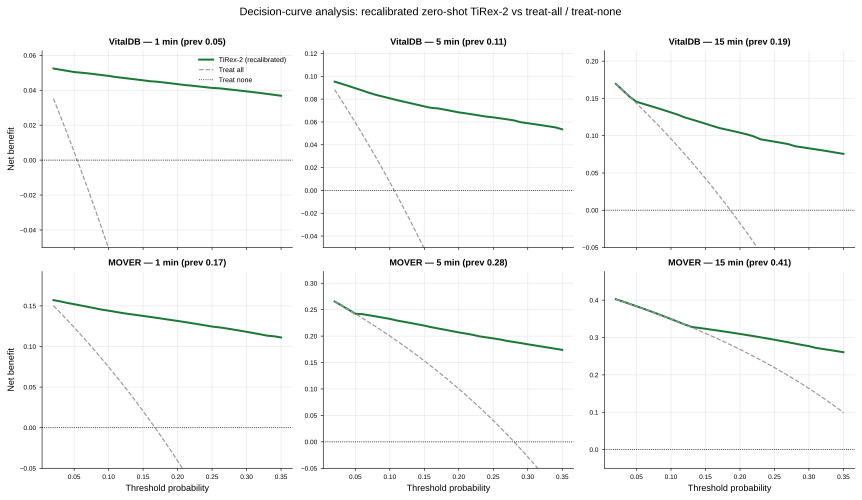
\includegraphics[width=\textwidth]{figs/FigS_decision_curves.png}
\caption{\textbf{Decision-curve analysis of recalibrated zero-shot TiRex-2, both cohorts.} Net benefit versus threshold probability at 1, 5 and 15~min on VitalDB (top) and MOVER (bottom), for the isotonic-recalibrated TiRex-2 risk against the two default strategies, treat-all (dashed) and treat-none (net benefit 0, dotted). The recalibrated model exceeded both references across essentially the whole clinically plausible threshold range on VitalDB (100\% of 2--35\% thresholds at 1 and 5~min; 91\% at 15~min) and over most of the range on MOVER (100\%/88\%/68\% at 1/5/15~min), the narrowing at MOVER 15~min reflecting the very high event prevalence (41\%), which raises the treat-all reference. Curves use the held-out test split with the isotonic map fitted on each cohort's disjoint development split.}
\label{fig:dca}
\end{figure}

% ==================== Explainability: what the zero-shot representations encode ====================
% ---------- Supplementary Figure : UMAP of per-window representations, VitalDB ----------
\begin{figure}[ht]
\centering
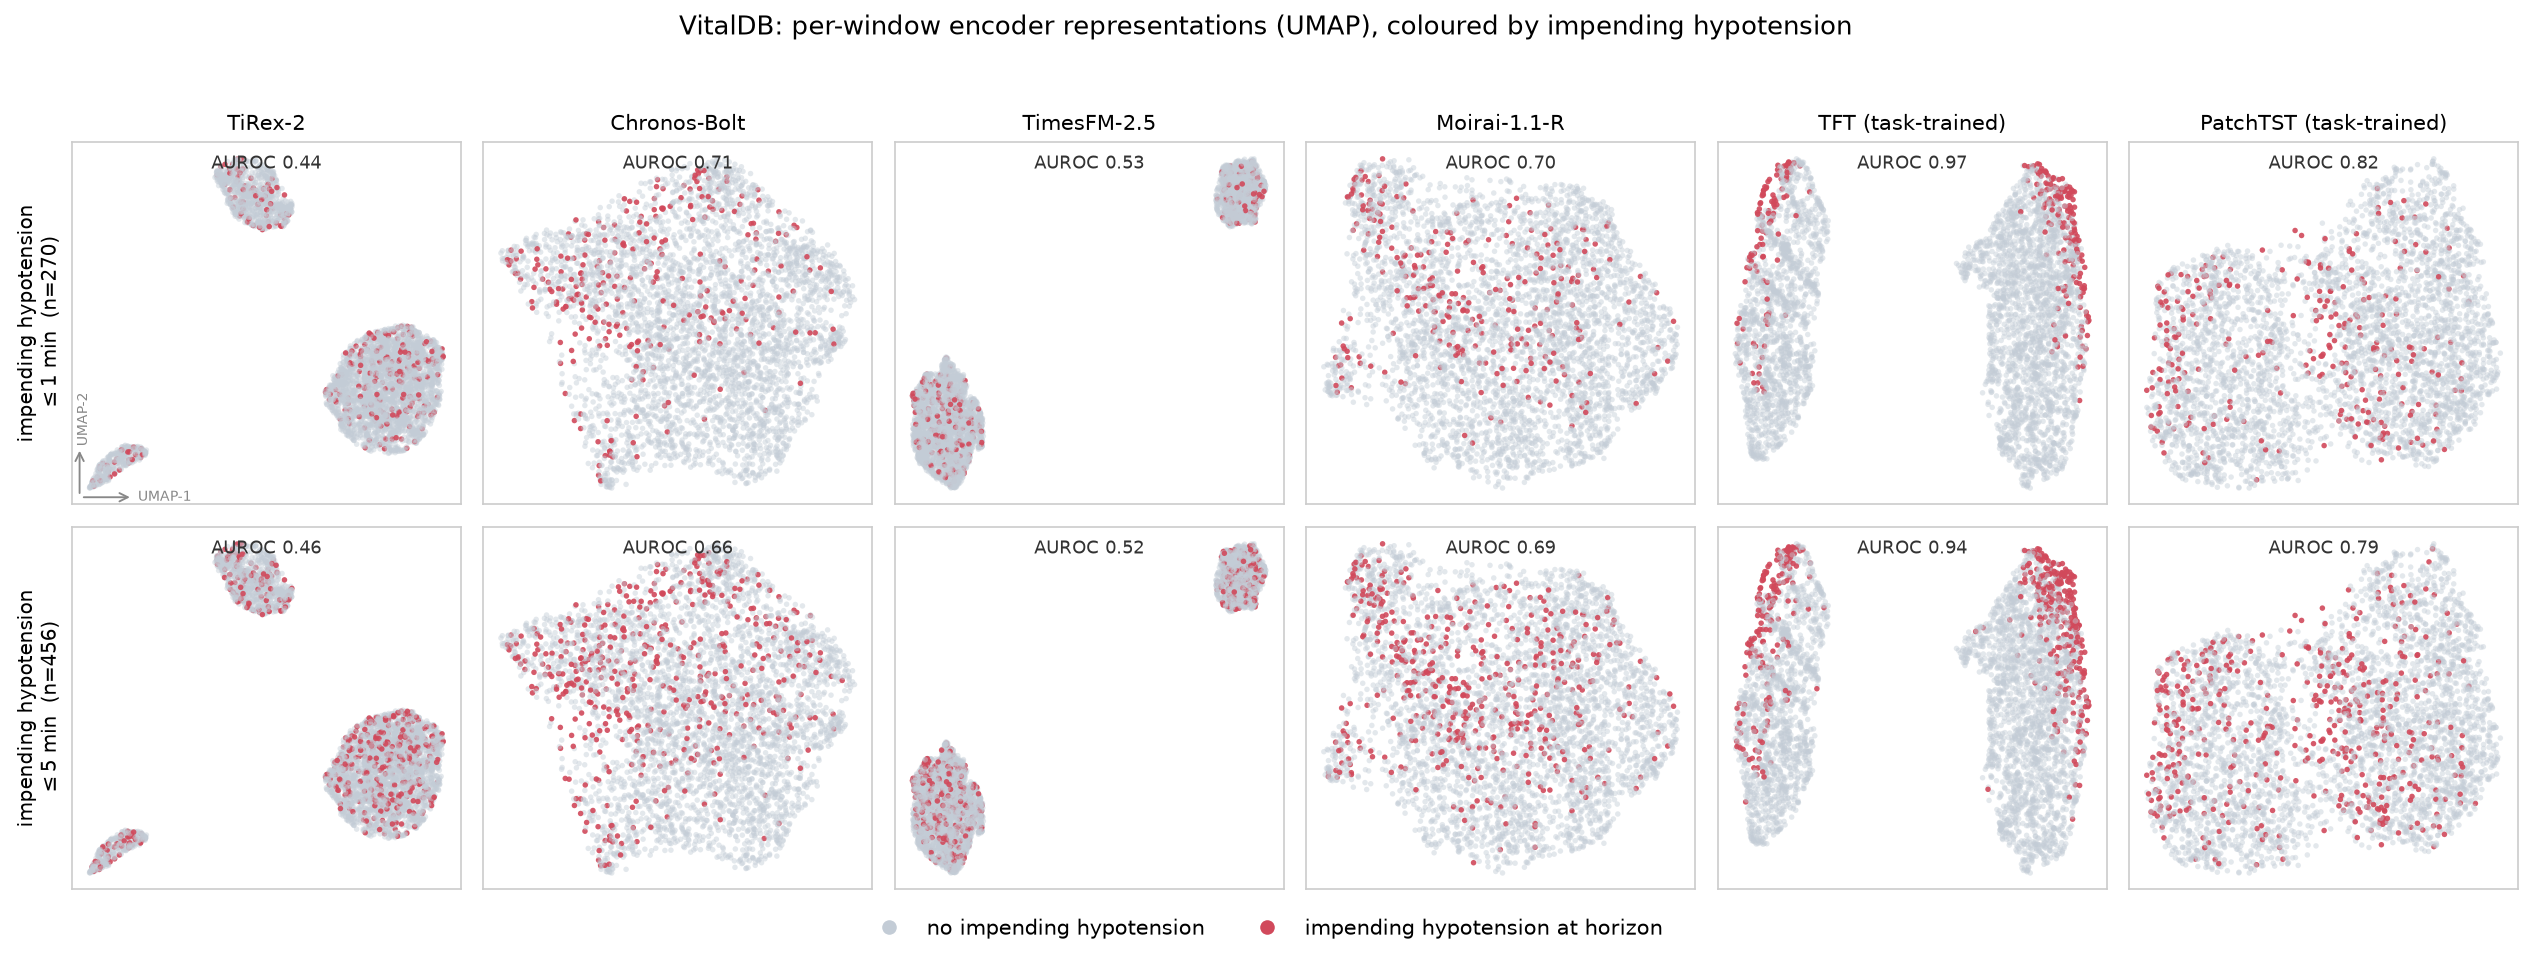
\includegraphics[width=\textwidth]{figs/FigS_umap_vitaldb.png}
\caption{\textbf{Per-window encoder representations on VitalDB, projected with UMAP and coloured by impending hypotension.} Each point is one forecast window; its position is a 2-D UMAP projection of that model's pooled penultimate-layer representation (standardised, Euclidean), and its colour marks whether MAP fell below 65~mmHg within the stated horizon (top row 1~min, bottom row 5~min; identical 4{,}000-window subsample across all models). The per-panel value is the AUROC of a subject-grouped linear probe for the same label (Supplementary Table~\ref{tab:probe_hypo}). Two distinct structures should not be conflated. (i)~The \emph{clinical} label appears as a diffuse colour \emph{gradient}, not as discrete clusters: red concentrates in a region of the manifold for the task-trained models (TFT, PatchTST) and, more weakly, for the univariate zero-shot models (Chronos, Moirai), but is spread at base rate for TiRex-2 and TimesFM-2.5. (ii)~The \emph{discrete} groupings visible in some panels (TiRex-2, TimesFM-2.5 split into separated islands) are \emph{not} clinical---they reflect embedding-activation magnitude or surgical context, not outcome (Supplementary Table~\ref{tab:cluster_char}). Notably the best forecaster, TiRex-2, shows the weakest colour gradient of all six models.}
\label{fig:umap_vitaldb}
\end{figure}

% ---------- Supplementary Figure : UMAP of per-window representations, MOVER ----------
\begin{figure}[ht]
\centering
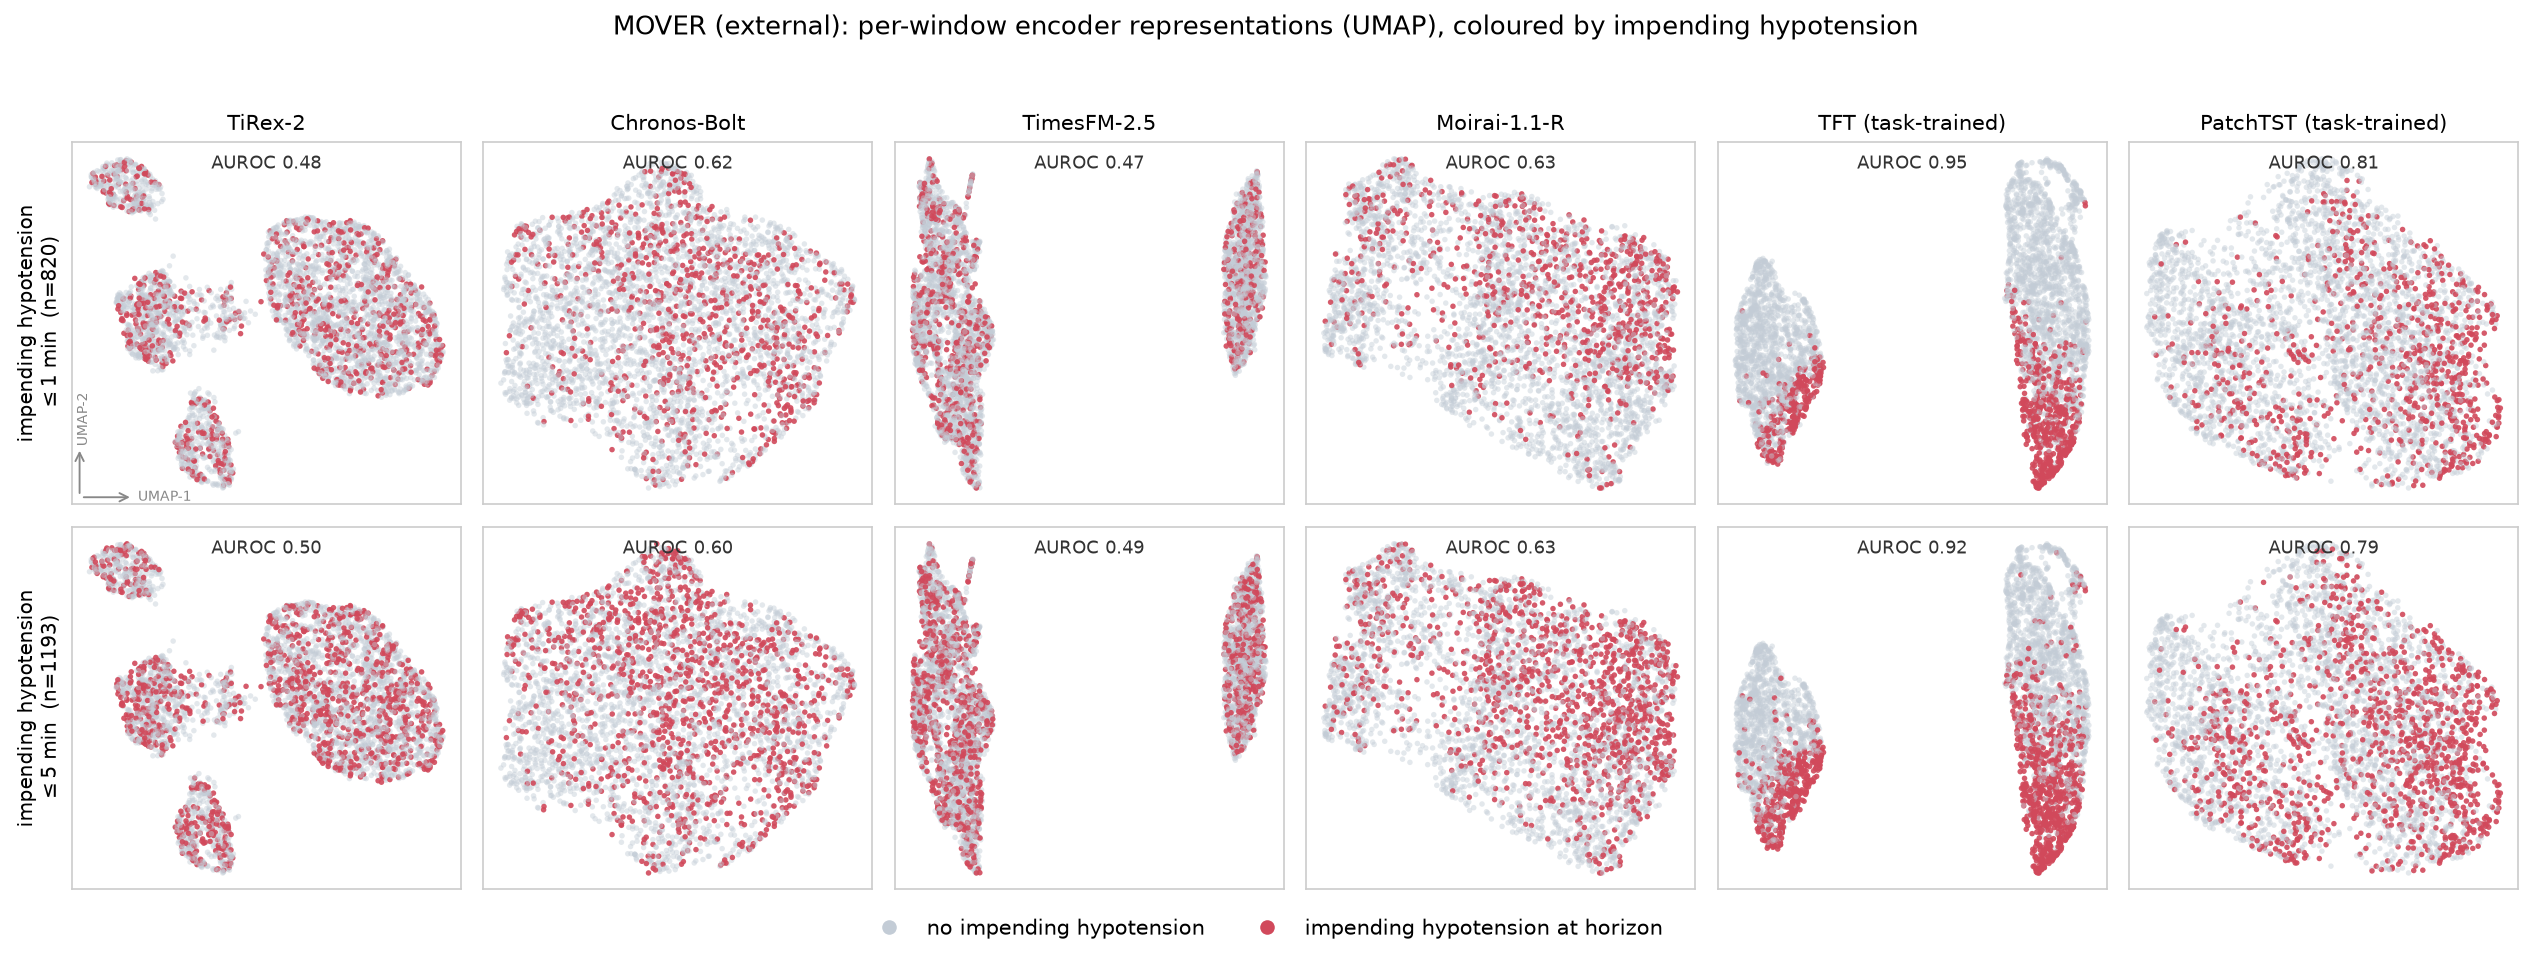
\includegraphics[width=\textwidth]{figs/FigS_umap_mover.png}
\caption{\textbf{Per-window encoder representations on the external MOVER cohort, projected with UMAP.} As Supplementary Fig.~\ref{fig:umap_vitaldb}, on the independent MOVER cohort (3{,}999-window subsample; 60~s cadence; higher hypotension prevalence). The pattern replicates externally: the model ordering by colour-gradient strength (probe AUROC) is unchanged---task-trained $>$ univariate zero-shot $>$ TiRex-2/TimesFM-2.5 at chance---and the non-clinical discrete islands persist for the same models.}
\label{fig:umap_mover}
\end{figure}

% ---------- Supplementary Figure : RSA / linear CKA ----------
\begin{figure}[ht]
\centering
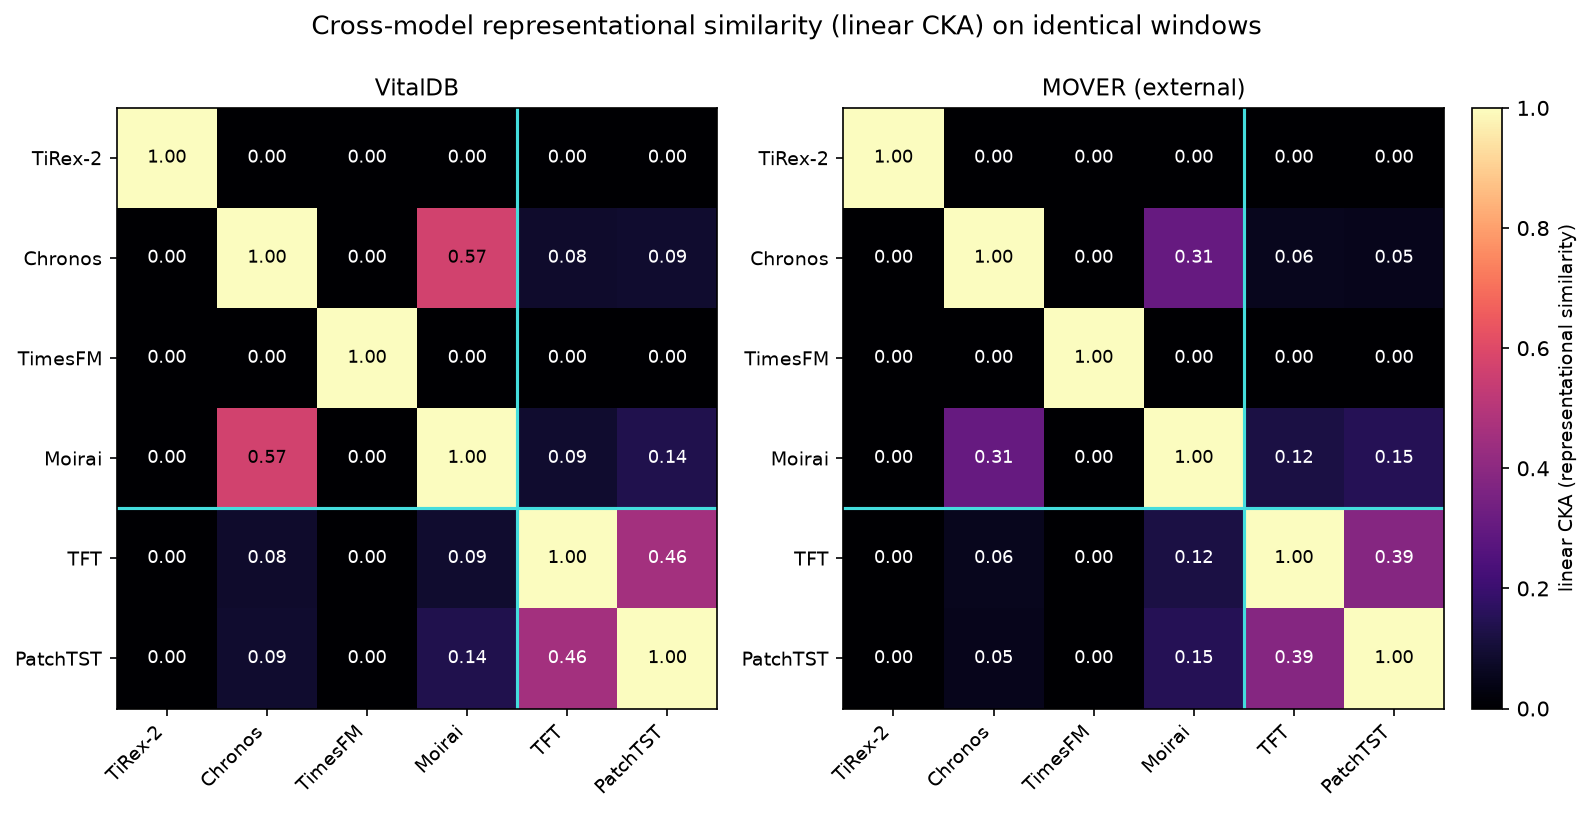
\includegraphics[width=\textwidth]{figs/FigS_rsa_cka.png}
\caption{\textbf{Cross-model representational similarity (linear CKA) on identical windows, both cohorts.} Linear centred kernel alignment between every pair of models' per-window representations, computed on the identical window subsample (dimension-agnostic, so it compares representations of different width). Cyan lines separate the zero-shot foundation models (upper-left block) from the task-trained baselines (lower-right). Cross-family similarity is near zero on both cohorts; the only substantial off-diagonal similarities are \emph{within} family---Chronos-Bolt$\leftrightarrow$Moirai (0.57 VitalDB) and TFT$\leftrightarrow$PatchTST (0.46)---while TiRex-2 and TimesFM-2.5 are nearly orthogonal to all other models. The four zero-shot models therefore do not share a common representational geometry, and none aligns with the task-trained models, even though several forecast comparably well.}
\label{fig:rsa_cka}
\end{figure}

% ---------- Supplementary Table : hypotension linear probe ----------
\begin{table}[ht]
\centering\footnotesize
\caption{\textbf{Linear separability of impending hypotension from per-window representations (subject-grouped probe).} AUROC (mean over 5 subject-grouped folds; per-fold s.d.\ $\leq$0.036 throughout) of an L2-regularised logistic probe predicting MAP$<$65~mmHg within each horizon from each model's frozen representation; no representation is fine-tuned. Area under the precision--recall curve is reported in the accompanying machine-readable table (\texttt{suppl\_probe\_hypotension.csv}). Windows are the identical subsample of Supplementary Figs.~\ref{fig:umap_vitaldb}--\ref{fig:umap_mover}, and folds are split by case so no subject appears in both train and test. Separability is a property of the \emph{representation}: it is highest for the task-trained models (which were optimised to expose exactly this label) and, among the zero-shot models, present but partial for the univariate Chronos-Bolt and Moirai and at chance for TiRex-2 and TimesFM-2.5. The ordering is stable across horizons and replicates on MOVER. Crucially it does not track forecasting skill---TiRex-2, the strongest forecaster, has the least task-separable representation.}
\label{tab:probe_hypo}
\begin{tabular}{llrrrrrr}
\toprule
& & \multicolumn{6}{c}{AUROC by horizon (min)} \\
\cmidrule(lr){3-8}
Cohort & Model & 1 & 2 & 3 & 5 & 10 & 15 \\
\midrule
\multicolumn{8}{l}{\textit{VitalDB (development)}}\\
& TiRex-2 & 0.441 & 0.455 & 0.462 & 0.464 & 0.479 & 0.485 \\
& Chronos-Bolt & 0.706 & 0.688 & 0.700 & 0.656 & 0.624 & 0.615 \\
& TimesFM-2.5 & 0.531 & 0.513 & 0.521 & 0.522 & 0.501 & 0.483 \\
& Moirai-1.1-R & 0.697 & 0.715 & 0.705 & 0.691 & 0.670 & 0.657 \\
& TFT (trained) & \textbf{0.974} & \textbf{0.964} & \textbf{0.954} & \textbf{0.939} & \textbf{0.911} & \textbf{0.892} \\
& PatchTST (trained) & 0.821 & 0.818 & 0.810 & 0.785 & 0.768 & 0.750 \\
\midrule
\multicolumn{8}{l}{\textit{MOVER (external)}}\\
& TiRex-2 & 0.485 & 0.486 & 0.503 & 0.504 & 0.481 & 0.482 \\
& Chronos-Bolt & 0.623 & 0.621 & 0.615 & 0.601 & 0.604 & 0.592 \\
& TimesFM-2.5 & 0.472 & 0.486 & 0.493 & 0.490 & 0.512 & 0.504 \\
& Moirai-1.1-R & 0.630 & 0.618 & 0.614 & 0.626 & 0.604 & 0.602 \\
& TFT (trained) & \textbf{0.951} & \textbf{0.938} & \textbf{0.925} & \textbf{0.915} & \textbf{0.896} & \textbf{0.884} \\
& PatchTST (trained) & 0.812 & 0.801 & 0.791 & 0.785 & 0.776 & 0.769 \\
\bottomrule
\end{tabular}
\end{table}

% ---------- Supplementary Table : continuous MAP trajectory probe ----------
\begin{table}[ht]
\centering\footnotesize
\caption{\textbf{Linear decodability of continuous hemodynamic state from per-window representations ($R^2$).} Cross-validated $R^2$ (subject-grouped ridge probe) predicting continuous mean arterial pressure quantities from each frozen representation: current MAP at the forecast origin, mean and minimum MAP over the next 5~min, mean MAP over the full horizon, and MAP slope over 5~min and the full horizon. Negative $R^2$ means the probe does worse than predicting the mean. This is the construct-valid test for a forecaster---whether its latent linearly encodes the hemodynamic trajectory---and the result is striking: only the task-trained TFT exposes MAP linearly ($R^2\!\approx\!0.8$--0.96 for current/near-future level), while the zero-shot foundation models are weak to negative, TiRex-2 included ($R^2\!\approx\!-0.08$, i.e.\ at chance). A forecaster's skill therefore resides in its full encoder$\rightarrow$decoder mapping conditioned on covariates, not in a linearly-decodable summary of its pooled penultimate state, which discards the temporal detail the forecast head uses.}
\label{tab:probe_traj}
\begin{tabular}{llrrrrrr}
\toprule
& & MAP & MAP +5 & MAP +5 & MAP +H & slope & slope \\
Cohort & Model & now & mean & min & mean & 5\,min & H \\
\midrule
\multicolumn{8}{l}{\textit{VitalDB (development)}}\\
& TiRex-2 & -0.08 & -0.08 & -0.08 & -0.09 & -0.07 & -0.08 \\
& Chronos-Bolt & 0.27 & 0.12 & 0.08 & -0.04 & -0.09 & -0.08 \\
& TimesFM-2.5 & -0.18 & -0.19 & -0.17 & -0.18 & -0.17 & -0.22 \\
& Moirai-1.1-R & 0.24 & 0.01 & 0.00 & -0.14 & -0.22 & -0.18 \\
& TFT (trained) & \textbf{0.81} & \textbf{0.78} & \textbf{0.70} & \textbf{0.70} & \textbf{0.19} & \textbf{0.30} \\
& PatchTST (trained) & 0.24 & 0.22 & 0.21 & 0.17 & 0.04 & 0.12 \\
\midrule
\multicolumn{8}{l}{\textit{MOVER (external)}}\\
& TiRex-2 & -0.09 & -0.09 & -0.10 & -0.09 & -0.09 & -0.07 \\
& Chronos-Bolt & 0.14 & -0.05 & -0.02 & -0.10 & -0.08 & -0.15 \\
& TimesFM-2.5 & -0.23 & -0.21 & -0.21 & -0.22 & -0.17 & -0.16 \\
& Moirai-1.1-R & 0.11 & -0.14 & -0.09 & -0.23 & -0.26 & -0.24 \\
& TFT (trained) & \textbf{0.96} & \textbf{0.73} & \textbf{0.73} & \textbf{0.66} & \textbf{0.09} & \textbf{0.14} \\
& PatchTST (trained) & 0.38 & 0.26 & 0.26 & 0.22 & 0.04 & 0.04 \\
\bottomrule
\end{tabular}
\end{table}

% ---------- Supplementary Table : cluster characterisation ----------
\begin{table}[ht]
\centering\footnotesize
\caption{\textbf{What the discrete groupings in the representation space encode.} For each model a 2-means split of the per-window representation is characterised by: its silhouette (how bimodal the representation is; higher = more clearly two groups), and the association of the split with candidate explanatory variables---window stratum and impending hypotension (adjusted mutual information, AMI), current MAP level and embedding L2-norm (AUROC of the split against the variable), surgical department (AMI, VitalDB only), and case purity (fraction of cases whose windows fall entirely in one group; high = a case-level attribute drives the split). No model's dominant split encodes the clinical outcome (AMI$_{\text{hypo}}\!\approx\!0$ throughout). Instead the strongly bimodal zero-shot models (TimesFM-2.5, TiRex-2) split on \emph{embedding magnitude} (norm AUROC~1.00), an activation-scale artifact; the task-trained models (TFT, PatchTST) split near-purely by \emph{case} on \emph{surgical department}; and Chronos-Bolt/Moirai are effectively unimodal (silhouette $\leq$0.17), their weak structure a gentle MAP-level gradient.}
\label{tab:cluster_char}
\begin{tabular}{llrrrrrrr}
\toprule
& & Split & \multicolumn{2}{c}{AMI} & \multicolumn{2}{c}{Split AUROC} & Case & AMI \\
\cmidrule(lr){4-5}\cmidrule(lr){6-7}
Cohort & Model & silh.\ & strat.\ & hypo & MAP lvl & emb.\ norm & purity & dept.\ \\
\midrule
\multicolumn{9}{l}{\textit{VitalDB (development)}}\\
& TiRex-2 & 0.47 & 0.00 & 0.00 & 0.51 & \textbf{1.00} & 0.58 & 0.00 \\
& Chronos-Bolt & 0.11 & 0.00 & 0.03 & 0.73 & 0.82 & 0.70 & 0.00 \\
& TimesFM-2.5 & \textbf{0.79} & 0.00 & 0.00 & 0.50 & \textbf{1.00} & 0.52 & 0.00 \\
& Moirai-1.1-R & 0.10 & 0.01 & 0.01 & 0.53 & 0.70 & 0.68 & 0.00 \\
& TFT (trained) & 0.23 & 0.01 & 0.00 & 0.50 & 0.56 & \textbf{0.99} & 0.26 \\
& PatchTST (trained) & 0.22 & 0.01 & 0.00 & 0.56 & 0.79 & 0.91 & 0.16 \\
\midrule
\multicolumn{9}{l}{\textit{MOVER (external)}}\\
& TiRex-2 & 0.29 & 0.00 & 0.00 & 0.51 & 0.63 & 0.64 & --- \\
& Chronos-Bolt & 0.06 & 0.00 & 0.02 & 0.67 & 0.57 & 0.51 & --- \\
& TimesFM-2.5 & \textbf{0.82} & 0.00 & 0.00 & 0.51 & \textbf{1.00} & 0.38 & --- \\
& Moirai-1.1-R & 0.17 & 0.00 & 0.02 & 0.51 & 0.94 & 0.59 & --- \\
& TFT (trained) & 0.42 & 0.00 & 0.00 & 0.52 & 0.50 & \textbf{0.89} & --- \\
& PatchTST (trained) & 0.20 & 0.00 & 0.04 & 0.67 & 0.58 & 0.74 & --- \\
\bottomrule
\end{tabular}
\end{table}

% ---------- Supplementary Table : TRIPOD+AI reporting checklist ----------
\clearpage
{\footnotesize
\setlength{\LTleft}{0pt}\setlength{\LTright}{0pt}
\begin{longtable}{@{}p{0.055\textwidth} p{0.40\textwidth} p{0.47\textwidth}@{}}
\caption{\textbf{TRIPOD+AI reporting checklist.} Adherence of this study to the
TRIPOD+AI statement for the transparent reporting of clinical-prediction models that use
regression or machine-learning methods \citep{Collins2024}. Each item is mapped to the
section where it is addressed. ``Section'' refers to the numbered sections of the main text
unless a Supplement item is named. Because the foundation models are applied \emph{zero-shot}
(no task-specific training, no development sample and no fitted parameters), the model-development
items (12--16) are reported as they apply to the two task-trained baselines and, for the
zero-shot exemplars, as ``not applicable --- pretrained, applied without fitting.''}
\label{tab:tripod}\\
\toprule
\textbf{Item} & \textbf{TRIPOD+AI checklist item} & \textbf{Reported in} \\
\midrule
\endfirsthead
\multicolumn{3}{@{}l}{\textit{Supplementary Table~\ref{tab:tripod} (continued)}}\\
\toprule
\textbf{Item} & \textbf{TRIPOD+AI checklist item} & \textbf{Reported in} \\
\midrule
\endhead
\midrule
\multicolumn{3}{@{}r}{\textit{continued on next page}}\\
\endfoot
\bottomrule
\endlastfoot

\multicolumn{3}{@{}l}{\textbf{Title and abstract}}\\
1 & Identify the study as developing/validating a prediction model, the target population and the outcome. & Title; Abstract. \\
2 & Structured summary of objectives, data, methods, results and conclusions. & Abstract. \\
\multicolumn{3}{@{}l}{\textbf{Introduction}}\\
3a & Background and rationale, referencing existing models. & Introduction (Kapral, Zhu, HPI as comparators). \\
3b & Objectives, specifying development and/or validation. & Introduction (three questions: paradigm rivalry, differentiator, external replication). \\
\multicolumn{3}{@{}l}{\textbf{Methods --- data}}\\
4a & Source of data (cohort, registry) and rationale, separately for development and validation. & \S4.1 (VitalDB development; MOVER external validation). \\
4b & Study dates (start of accrual, end of follow-up). & \S4.1; source-dataset citations \citep{Lee2022,Samad2023}. \\
5a & Study setting, eligibility criteria, inclusion cascade. & \S4.1 (case-flow funnel; Fig.~1b). \\
5b & Details of treatments received, where relevant. & \S4.1, \S4.3 (remifentanil / propofol infusion as covariates). \\
6a & Outcome definition and how/when assessed. & \S4.3 (MAP\,$<$\,65~mmHg within the forecast horizon). \\
6b & Any actions to blind assessment of the outcome. & \S4.3 (outcome computed algorithmically from the arterial-MAP trace; no adjudication). \\
7a & Predictors/features used, how and when measured. & \S4.3, \S4.2 (30-min context of MAP $+$ covariates; resampling). \\
7b & Any actions to blind predictor assessment. & Not applicable (fully automated feature construction). \\
8 & Sample size and how it was arrived at. & \S4.1 (all eligible cases; 2{,}708 VitalDB / 1{,}827 MOVER; no a-priori size calculation --- full available cohort). \\
9 & Missing-data handling. & \S4.1--4.2 (coverage gates; artefact removal; despiking; per-window eligibility). \\
\multicolumn{3}{@{}l}{\textbf{Methods --- model}}\\
10a & How predictors were handled in the analysis. & \S4.2--4.3 (resampling to fixed cadence; covariate channels). \\
10b & Model type, building procedure, predictor selection, internal validation. & \S4.4 (zero-shot FMs applied without fitting; TFT/PatchTST trained by 5-fold subject-level cross-validation). \\
11 & How predictions were calculated / risk score obtained. & \S4.3--4.4 (quantile forecasts; threshold-crossing risk); \S2.5 recalibration. \\
12 & AI/ML specifics: architecture, hyperparameters, training, compute, software. & \S4.4, \S4.6 (architectures, hyperparameters); \S4.6 (A100 hardware); \S4.9 (software/reproducibility). \\
13 & Fairness / subgroup considerations in model building. & \S2.5, Fig.~5d (VitalDB and MOVER external subgroup forest plots). \\
14 & Performance measures and rationale. & \S4.5 (AUROC, AUPRC, CRPS, MAE, calibration, decision curve). \\
15 & Model updating / recalibration, if any. & \S2.5 (post-hoc isotonic recalibration; transportability). \\
16 & Analysis of model performance, including comparison. & \S2.2--2.6 (FM ranking, vs task-trained, external transfer, naive floor). \\
\multicolumn{3}{@{}l}{\textbf{Methods --- validation and open science}}\\
17 & Methods for external validation. & \S2.6, \S4.5 (MOVER external; in-domain OOF vs transferred). \\
18 & Risk-of-bias / applicability assessment approach. & \S3 Limitations (optimistic-upper-bound, pretraining contamination, cadence). \\
\multicolumn{3}{@{}l}{\textbf{Results}}\\
19a & Participant flow (development and validation). & Fig.~1b (two-cohort funnel); Table~1. \\
19b & Participant characteristics, including outcome prevalence. & Table~1 (both cohorts; prevalence by horizon). \\
20 & Model specification / performance of final model. & \S2.2--2.6; Tables~2--4; Figs.~2--6. \\
21 & Model performance with confidence intervals; subgroups. & Tables~2--4 (case-clustered bootstrap 95\% CIs); Fig.~5d (VitalDB and MOVER subgroup forest plots). \\
22 & Comparison with other models / literature. & \S2.3, Tables (Kapral, Zhu literature values clearly marked). \\
\multicolumn{3}{@{}l}{\textbf{Discussion}}\\
23 & Interpretation, in context of objectives and prior evidence. & \S3 (Relation to SOTA; where task-trained lead; naive floor). \\
24 & Limitations (bias, generalisability). & \S3 Limitations. \\
25 & Usability in practice and implications for clinical use. & \S2.4--2.5, \S3 (decision-curve; early-warning framing; prospective evaluation required). \\
\multicolumn{3}{@{}l}{\textbf{Other information}}\\
26 & Supplementary information / protocol availability. & \S4.9; Supplementary Information. \\
27 & Funding and role of funders. & Funding statement. \\
\multicolumn{3}{@{}l}{\textbf{Open science / declarations}}\\
O1 & Data availability. & Data availability statement (VitalDB, MOVER). \\
O2 & Code availability. & Code availability statement (Zenodo archive on acceptance; maintained GitHub repo). \\
O3 & Model availability (weights). & Model availability statement (Hugging Face checkpoints, method-paper citations). \\
O4 & Competing interests. & Competing interests statement. \\
O5 & Use of AI tools. & Use of AI tools statement. \\
\end{longtable}
}

